\documentclass{article}

\title{
\textbf{pacman-racket} \\
A pragmatic implementation of Pacman in Racket
}

\author{
    Alessandro Zanzi,
    Filippo Piloni,\\
    Jeferson Morales Mariciano,
    Paolo Deidda
}
\date{
USI \\
Faculty of Informatics \\
[\baselineskip]  2021/2022
}


\begin{document}
%%%%%%%%%%%%%%%%%%%%%%%
%%%%%%%%%%%%%%%%%%%%%%%
%%%%%%%%%%%%%%%%%%%%%%%
\begin{titlepage}
\maketitle

\end{titlepage}
 %%%%%%%%%%%%%%%%%%%%%%%
 %%%%%%%%%%%%%%%%%%%%%%%
 %%%%%%%%%%%%%%%%%%%%%%%
 \begin{abstract}
Conceptualization, research and thinking out-of-the-box
to implement the well-known classic Pacman game
using the Racket functional programming language.
 \end{abstract}
\clearpage
%%%%%%%%%%%%%%%%%%%%%%%
%%%%%%%%%%%%%%%%%%%%%%%
%%%%%%%%%%%%%%%%%%%%%%%
 \tableofcontents
 \clearpage
 %%%%%%%%%%%%%%%%%%%%%%%
 %%%%%%%%%%%%%%%%%%%%%%%
 %%%%%%%%%%%%%%%%%%%%%%%
 \section{Analysis}
 
 \hspace{0.5cm}\textbf{Modularity}\\
 In order for the group to work in parallel on the project we created several files on which each of us worked simultaneously. These files were then interconnected with the built in function of Racket "require" followed by the name of the file.
 
 %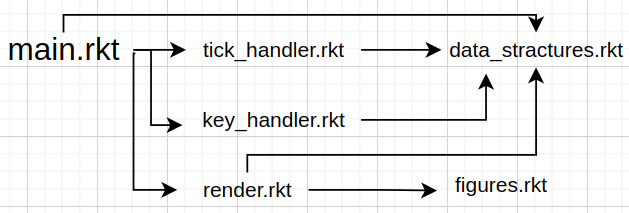
\includegraphics{images/dependency_three.png}
 
 
 \textbf{Bottom-up approach}\\
 We developed the code decomposing the functions needed in the simplest possible problems, we then conveyed them in higher grade functions. This allowed a design recepie with more tests making the debugging process easier.
 
 \textbf{Game logic}\\
The player must guide a yellow spherical creature, called Pac-Man, making it eat all the numerous dots scattered inside the maze and, in doing so, he must avoid being touched by four ghosts, or the game will be over. In order to make the game easier for the player, there are four "power pills" in the corners of the screen that turn the situation making the ghosts unable to touch Pac-Man. Each dot taken will increase the score of 10 points instead the cherries worth 100 points.

 %%%%%%%%%%%%%%%%%%%%%%%
 %%%%%%%%%%%%%%%%%%%%%%%
 %%%%%%%%%%%%%%%%%%%%%%%
 \section{Sofware design}
 \subsection{Tools}
 \hspace{0.5cm}\LaTeX \\
 Used for the user guide\\
 
 \textit{Flowchart}\\
 Used to create the dependency threes so each member of the group had a clear view of the whole project.
 

 \subsection{UI}
%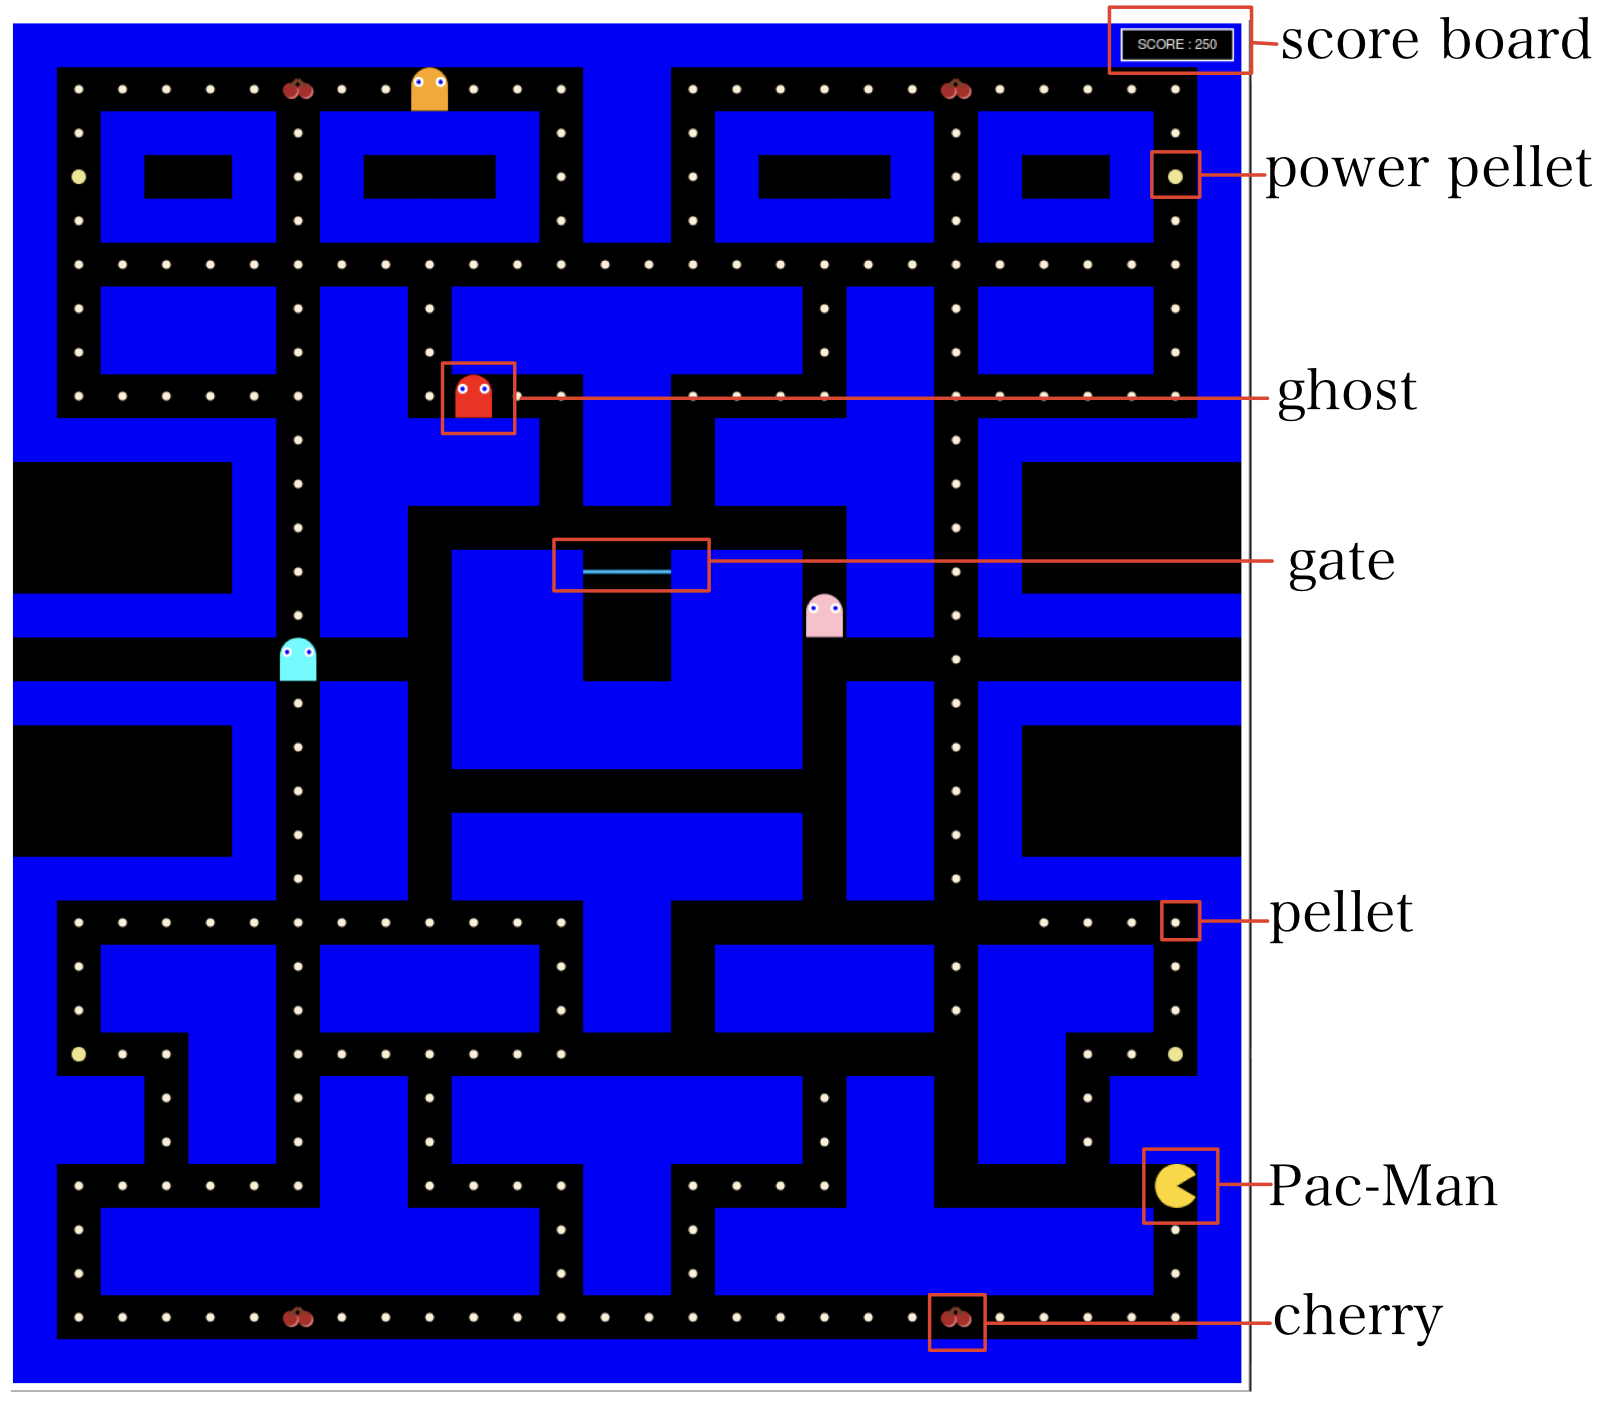
\includegraphics{./images/user_interface.png}

%%%%%%%%%%%%%%%%%%%%%%%
%%%%%%%%%%%%%%%%%%%%%%%
%%%%%%%%%%%%%%%%%%%%%%%
 \section{Software Development}
 \subsection{Tools}
 
 racket ling progr
 
 drRacket IDE
 
 
 VCS Git \\
 
 
Hosting Github
luogo fisico in github servers

\subsection{Libraries}
Universe \\
Image

%%%%%%%%%%%%%%%%%%%%%%%
%%%%%%%%%%%%%%%%%%%%%%%
%%%%%%%%%%%%%%%%%%%%%%%
 \section{Usage}
 
 ==> run

%%%%%%%%%%%%%%%%%%%%%%%
%%%%%%%%%%%%%%%%%%%%%%%
%%%%%%%%%%%%%%%%%%%%%%%

\end{document}
